\section{Xây dựng bộ xử lý lỗi}
\label{ch3:err-handler}

    Một thành phần không kém phần quan trọng trong quá tình thông dịch là bộ xử lý lỗi. Bộ xử lý lỗi sẽ giúp thông dịch hiển thị thông báo lỗi khi có lỗi xảy ra trong quá trình thông dịch. Bộ xử lý lỗi sẽ giúp thông dịch hiển thị thông báo lỗi cụ thể, giúp người dùng dễ dàng xác định lỗi và sửa lỗi.

\begin{figure}[H]
    \centering
    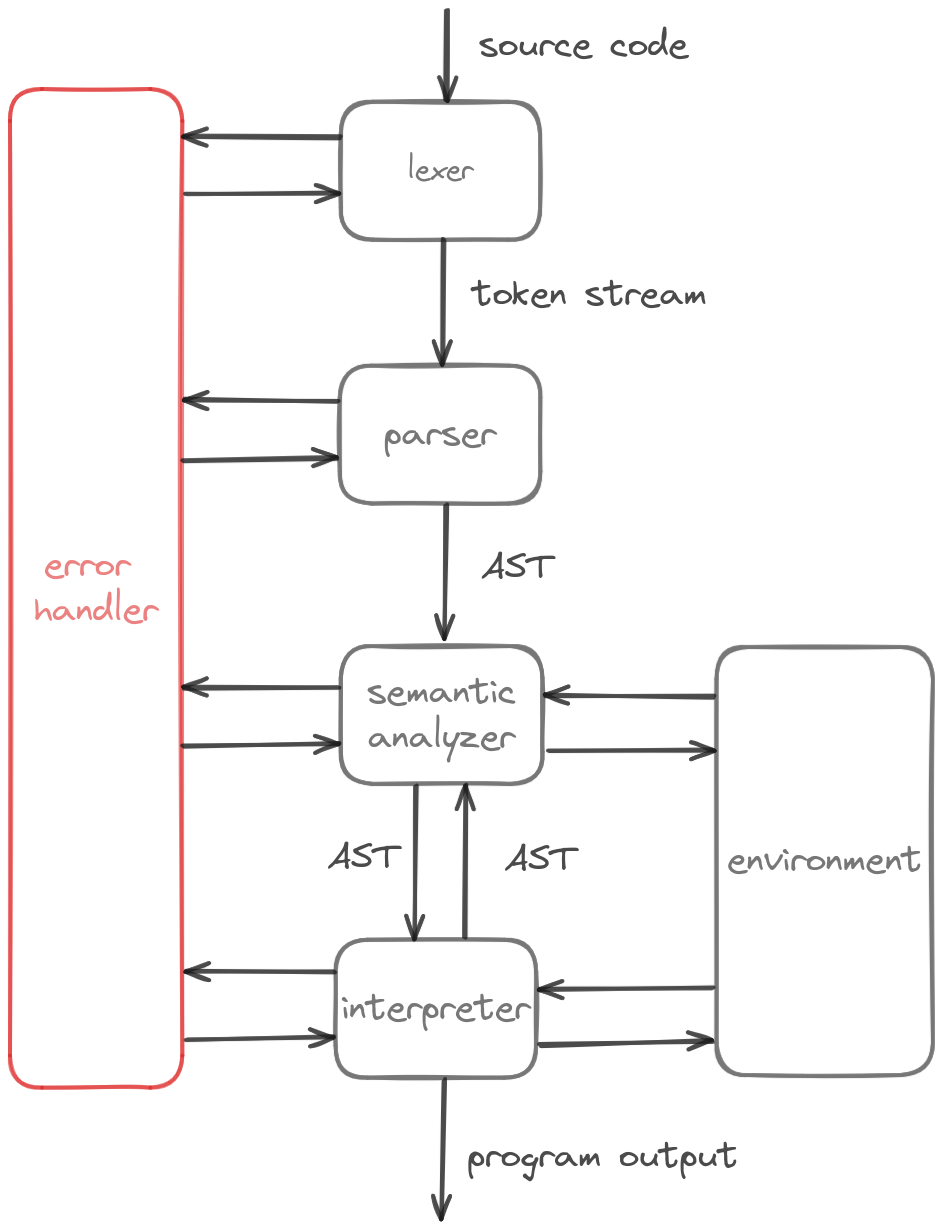
\includegraphics[scale=0.4]{error-handler-pos.png}
    \caption{Bộ xử lý lỗi trong cấu trúc của trình thông dịch Pandora}
\end{figure}

Dựa vào hình trên, ta có thể thấy quá trình xử lý lỗi được diễn ra tại mọi bước trong quá trình thông dịch. Khi có lỗi xảy ra, thông dịch sẽ gọi hàm xử lý lỗi để hiển thị thông báo lỗi cụ thể. Bộ xử lý lỗi sẽ được quản lý bởi một đối tượng là \texttt{ErrorHandler} (được định nghĩa trong \kw{src/error\_handler.rs}) như sau:

\begin{lstlisting}[]
pub struct ErrorHandler {
    pub file: Arc<SourceFile>,
}
\end{lstlisting}

Trong đó, \texttt{file} là một đối tượng \texttt{SourceFile} được chia sẻ giữa các thành phần trong trình thông dịch. \texttt{SourceFile} chứa toàn bộ nội dung của tệp tin chương trình. Khi có lỗi xảy ra, thông dịch sẽ gọi hàm xử lý lỗi để hiển thị thông báo lỗi cụ thể. Với mỗi một tập tin chương trình, thông dịch sẽ tạo một đối tượng \texttt{ErrorHandler} riêng để xử lý lỗi. Tính đến thời điểm ngày 15/12/2024, bộ xử lý lỗi trong Pandora tiếp nhận xử lý tổng cộng 72 loại lỗi, mỗi loại lỗi sẽ có một mã lỗi và một thông báo lỗi cụ thể. Dưới đây là một số mã lỗi và thông báo lỗi cụ thể:

\noindent \textbf{Chương trình thiếu dấu đóng chú thích}:

\begin{lstlisting}[]
/* this is a comment

/* another opening comment

close the first one */
\end{lstlisting}

\noindent Kết quả:
\begin{figure}[H]
    \centering
    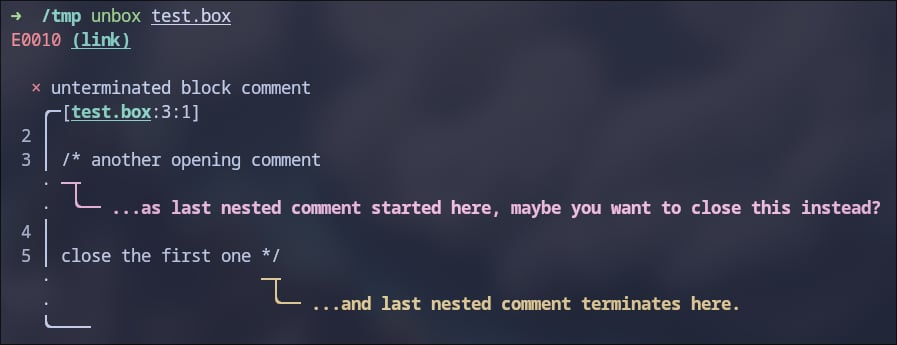
\includegraphics[scale=0.505]{ex-err-rt-1.jpg}
    \caption{Kết quả thực thi chương trình thiếu dấu đóng chú thích}
\end{figure}

\noindent Chi tiết mã lỗi:
\begin{figure}[H]
    \centering
    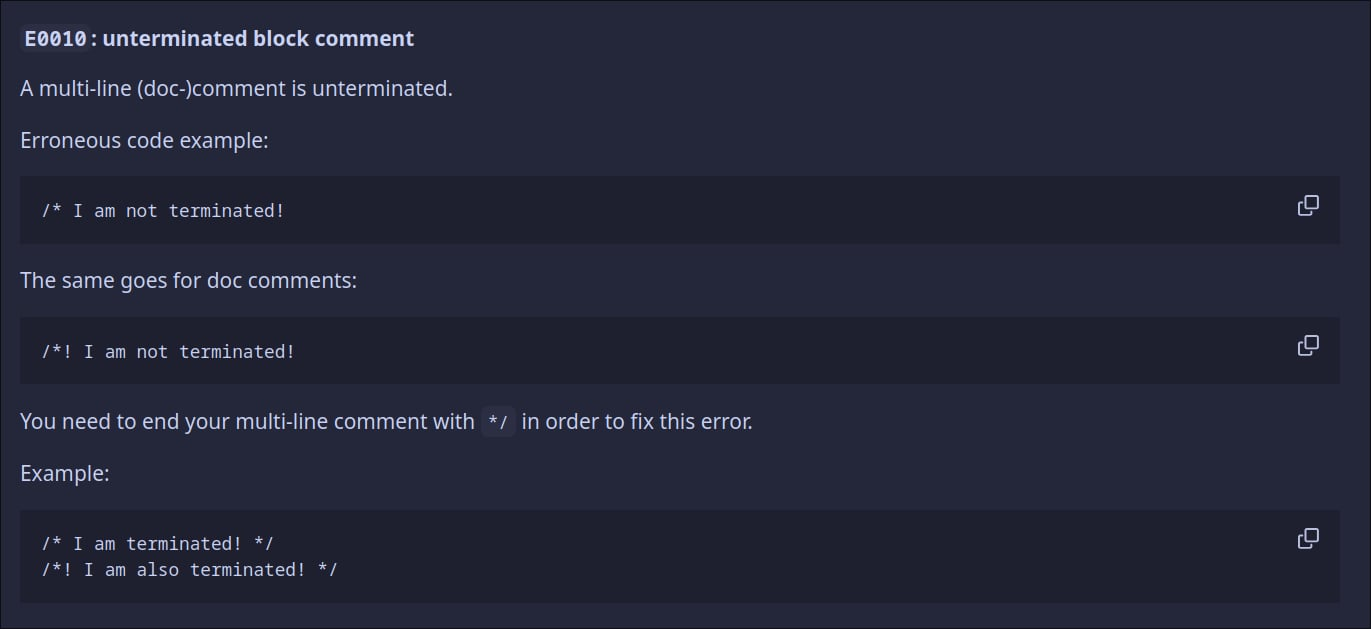
\includegraphics[scale=0.33]{ex-err-re-1.jpg}
    \caption{Chi tiết mã lỗi chương trình thiếu dấu đóng chú thích}
\end{figure}

\noindent \textbf{Chương trình sai tham số truyền vào}:

\begin{lstlisting}[]
fun abc(s: str) {
    println("unexpected args");
}

abc(1, true, "", 3);
\end{lstlisting}

\noindent Kết quả:
\begin{figure}[H]
    \centering
    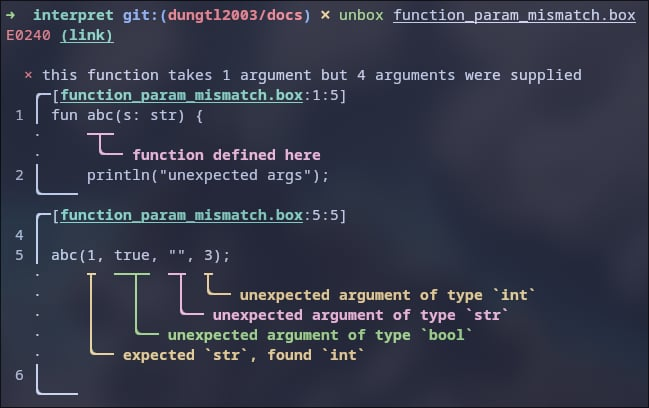
\includegraphics[scale=0.695]{ex-err-rt-2.jpg}
    \caption{Kết quả thực thi chương trình sai tham số truyền vào}
\end{figure}

\noindent Chi tiết mã lỗi:
\begin{figure}[H]
    \centering
    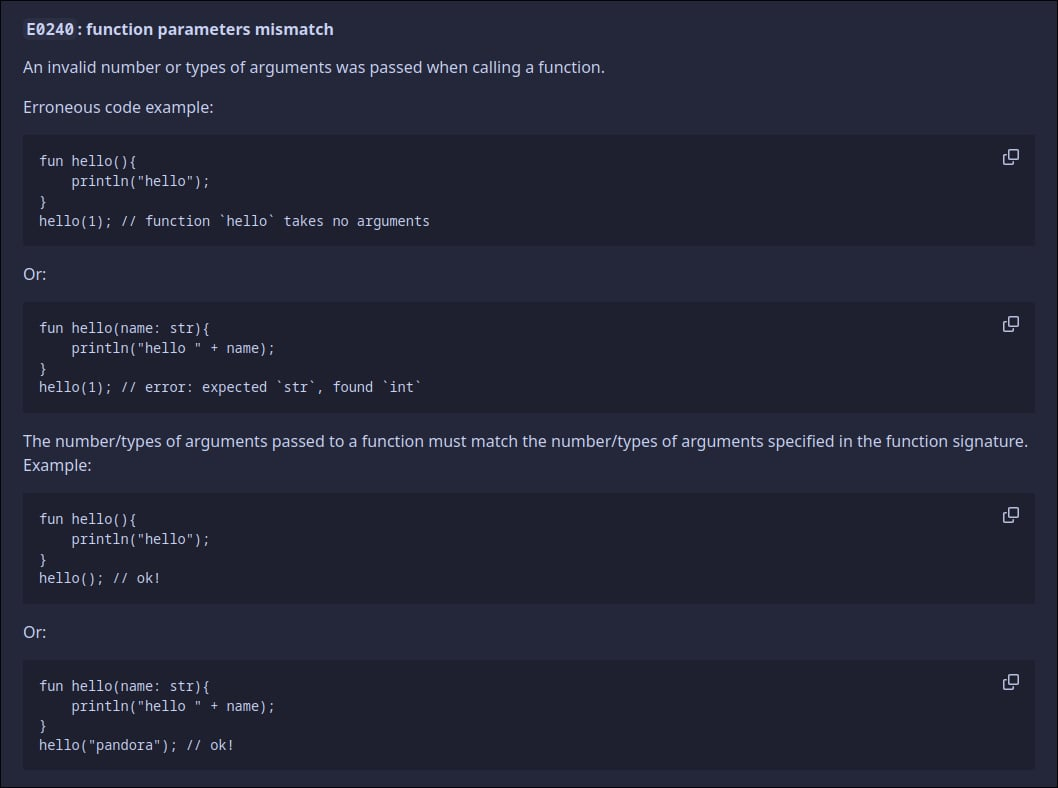
\includegraphics[scale=0.42]{ex-err-re-2.jpg}
    \caption{Chi tiết mã lỗi chương trình sai tham số truyền vào}
\end{figure}

\noindent \textbf{Chương trình hằng số không hợp lệ}:

\begin{lstlisting}[]
set a: int = 0b1234;
\end{lstlisting}

\noindent Kết quả:
\begin{figure}[H]
    \centering
    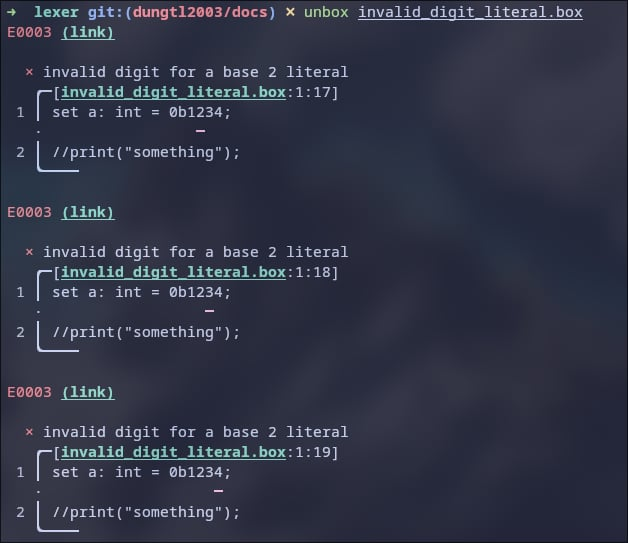
\includegraphics[scale=0.695]{ex-err-rt-3.jpg}
    \caption{Kết quả thực thi chương trình hằng số không hợp lệ}
\end{figure}

\noindent Chi tiết mã lỗi:
\begin{figure}[H]
    \centering
    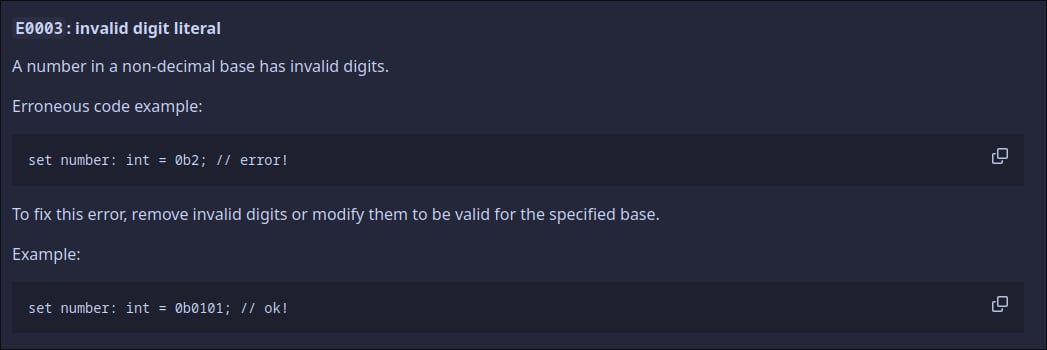
\includegraphics[scale=0.42]{ex-err-re-3.jpg}
    \caption{Chi tiết mã lỗi chương trình hằng số không hợp lệ}
\end{figure}

    Do bộ xử lý lỗi cần được sử dụng xuyên suốt quá trình thông dịch, để dễ dàng truy cập và sử dụng, nó sẽ được lưu vào đối tượng là \kw{Session} (được định nghĩa trong \kw{src/session.rs}). Đối tượng \kw{Session} có cấu trúc như sau:

\begin{lstlisting}[]
pub struct Session {
    pub error_type: ErrorType,
    pub error_handler: ErrorHandler,
}
\end{lstlisting}

    Trong đó, \kw{error\_handler} chính là bộ xử lý lỗi, còn \kw{error\_type} là loại lỗi. Lỗi trong Pandora sẽ được chia làm hai loại chính: \kw{Recoverable} (có thể khôi phục) và \kw{Unrecoverable} (không thể khôi phục được). Với loại lỗi có thể khôi phục được, bộ xử lý hiện tại chỉ cần cung cấp bộ xử lý lỗi một số thông tin cần thiết về loại lỗi hiện tại rồi tiếp tục thực hiện công việc của mình. Còn đối với lỗi không thể khôi phục được, ngay sau khi thông báo lỗi thông qua bộ xử lý lỗi, quá trình thông dịch sẽ kết thúc. Ta sẽ phân tích qua cách thức hoạt động của bộ xử lý lỗi trong từng giai đoạn của quá trình thông dịch.    

\subsection{Xử lý lỗi trong quá trình phân tích từ vựng}

    Trong quá trình phân tích từ vựng, mỗi khi bộ phân tích từ vựng gặp một lỗi, nó sẽ thông báo lỗi thông qua bộ xử lý lỗi. Bộ xử lý lỗi sẽ hiển thị thông báo lỗi cụ thể và vị trí lỗi trong tệp tin chương trình. Từ đố sai đó sẽ được tính vào loại từ tố lỗi và bỏ qua. Một số lỗi phổ biến trong quá trình phân tích từ vựng bao gồm: từ tố không hợp lệ, hằng số không hợp lệ, ký tự không hợp lệ, ... Trong đó, có một số lỗi không thể khôi phục được, ví dụ như lỗi chỉ có một dấu nháy kép. Khi gặp lỗi này, Bộ xử lý lỗi sẽ thông báo lỗi và kết thúc quá trình thông dịch ngay sau đó.

\subsection{Xử lý lỗi trong quá trình phân tích cú pháp}

    Đây là giai đoạn xử lý lỗi phức tạp nhất trong quá trình thông dịch. Tất cả các lỗi tại giai đoạn này đều có thể khôi phục được. Một số khó khăn khi thông báo lỗi ở giai đoạn này là:

\begin{itemize}
    \item \textbf{Thông báo được nhiều loại lỗi khác nhau nhất có thể}. Ta có thể thông báo một loại lỗi ta tìm thấy rồi kết thúc quá trình thông dịch, nhưng điều này sẽ khiến người dùng phải chạy lại chương trình nhiều lần để sửa hết lỗi. Điều này sẽ làm giảm hiệu suất làm việc của người dùng.
    \item \textbf{Giảm thiểu việc thông báo lỗi dư thừa}. Sau khi thông báo một loại lỗi nào đó, bộ phân tích cú pháp sẽ tiếp tục làm việc. Tuy nhiên, một lỗi có thể làm ảnh hưởng đến toàn bộ cú pháp. Nếu không xử lý khéo léo, bộ phân tích cú pháp sẽ thông báo rất nhiều lỗi dư thừa, không liên quan đến vấn đề chính.
\end{itemize}

    Như vậy, ta muốn thông báo ra được nhiều loại lỗi nhất có thể, nhưng lại không muốn thông báo ra những lỗi do hệ quả của lỗi trước đó. Để giải quyết vấn đề này, ta sẽ sử dụng một chiến thuật khôi phục lỗi phổ biến là chế độ hoảng loạn (panic mode). 

    \textbf{Chế độ hoảng loạn} là một chiến thuật khôi phục lỗi phổ biến trong quá trình phân tích cú pháp. Khi gặp lỗi, bộ phân tích cú pháp sẽ bỏ qua tất cả các từ tố cho đến khi gặp một từ tố nằm trong tập hợp các từ tố \textbf{đồng bộ} (synchronous token). Quá trình này được gọi là quá trình \textbf{đồng bộ hóa} (synchronization). Khi gặp một từ tố đồng bộ, chẳng hạn như \kw{;}, bộ phân tích cú pháp sẽ tiếp tục phân tích từ tố tiếp theo như bình thường. Thực hiện điều này sẽ có thể khiến bộ phân tích cú pháp bỏ qua một số lỗi, nhưng nó sẽ giúp giảm thiểu việc thông báo lỗi dư thừa. Để dễ hình dung cách xử lý lỗi ở giai đoạn này, ta sẽ xem xét một số ví dụ sau:

\begin{lstlisting}[]
set a = 1 3 x  y;

when a => 4 5 6 {
    a = b c e
    set a = 1
}

4 5
\end{lstlisting}

    Ở câu lệnh đầu tiên, ta có thể thấy người dùng đang cố thực hiện khởi tạo một biến \kw{a}. Tuy nhiên, cú pháp của lệnh khởi tạo yêu cầu sau tên biến cần kiểu dữ liệu (xem chi tiết cú pháp câu lệnh ở phần TODO), mà bộ phân tích cú pháp lại bắt gặp ký tự \kw{=}. Vì vậy, bộ phân tích cú pháp sẽ gửi thông tin lỗi cho bộ xử lý lỗi, đồng thời sẽ vào chế độ hoảng loạn. Vào lúc này, bộ phân tích cú pháp sẽ bỏ qua các ký tự dư thừa như \kw{1}, \kw{3}, \kw{x}, \kw{y} do chúng không phải các từ tố nằm trong danh sách các từ tố đồng bộ. Đến khi gặp ký tự \kw{;}, do nó có thuộc danh sách từ tố đồng bộ nên quá trình đồng bộ sẽ kết thúc. Bộ phân tích cú pháp sẽ quay lại chế độ bình thường và tiếp tục đọc câu lệnh tiếp theo. 

Từ tố tiếp theo sẽ xét lúc này là từ tố \kw{when}, người dùng ở đoạn này có thể đang muốn xây dựng câu lệnh rẽ nhánh. sau từ tố \kw{when} sẽ cần một biểu thức. Trong khi phân tích biểu thức, bộ phân tích cú pháp bắt gặp ký tự \kw{>} liền sau \kw{=}, và điều này là không hợp lệ. Tương tự như ban đầu, chế độ hoảng loạn được kích hoạt, các ký tự \kw{4}, \kw{5}, \kw{6} đều bị bỏ qua. Tới ký tự \kw{\{} thuộc danh sách từ tố đồng bộ, bộ phân tích cú pháp lại trở về trạng thái bình thường.

    Đối với câu lệnh đầu tiên trong khối lệnh, ký tự đầu tiên đọc được là \kw{a}, khiến cho câu lệnh rất có thể là một câu lệnh biểu thức. Ký tự sau \kw{a} là dấu \kw{=} khiến cho đây rất có thể là biểu thức gán. Tuy nhiên, sau phép gán chỉ được phép là một biểu thức khác, không thể nhiều hơn. Vì vậy, tương tự như hai lần trên, các ký tự \kw{c}, \kw{e} lần lượt bị bỏ qua cho tới từ khóa \kw{set}. 

Khi gặp từ khóa \kw{set}, trường hợp lại giống như câu lệnh đầu tiên, ký tự \kw{1} bị bỏ qua cho tới ký tự \kw{\}} (một trong những ký tự đồng bộ).

    Cuối cùng, khi bộ phân tích cú pháp gặp ký tự \kw{4} (có thể là một câu lệnh biểu thức), và sau \kw{4} là một ký tự không hợp lệ, bộ phân tích cú pháp sẽ thông báo lỗi và kết thúc quá trình thông dịch.

Ta có thể hiểu cả quá trình trên qua hình sau:  

\begin{figure}[H]
    \centering
    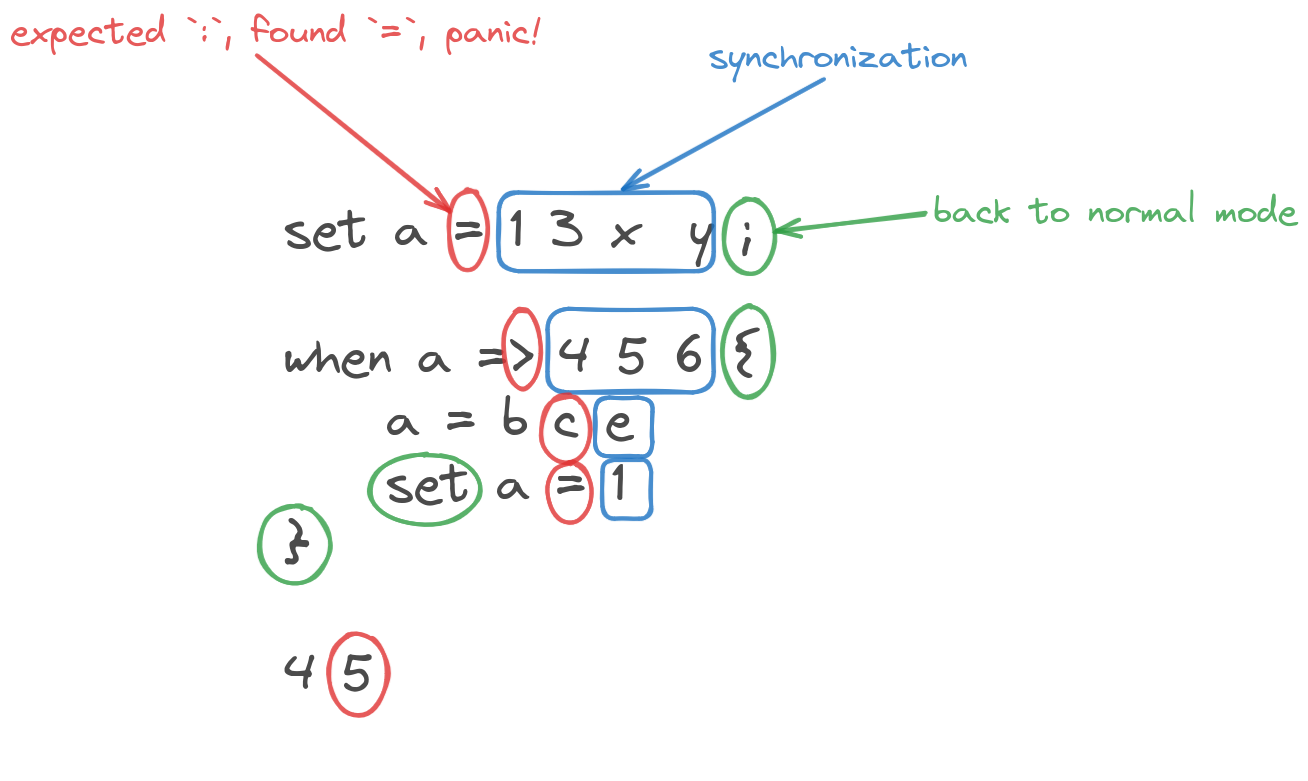
\includegraphics[scale=0.33]{panic-mode.png}
    \caption{Quá trình xử lý lỗi trong chế độ hoảng loạn}
\end{figure}

Và đây là kết quả thực thi chương trình trên:

\begin{figure}[H]
    \centering
    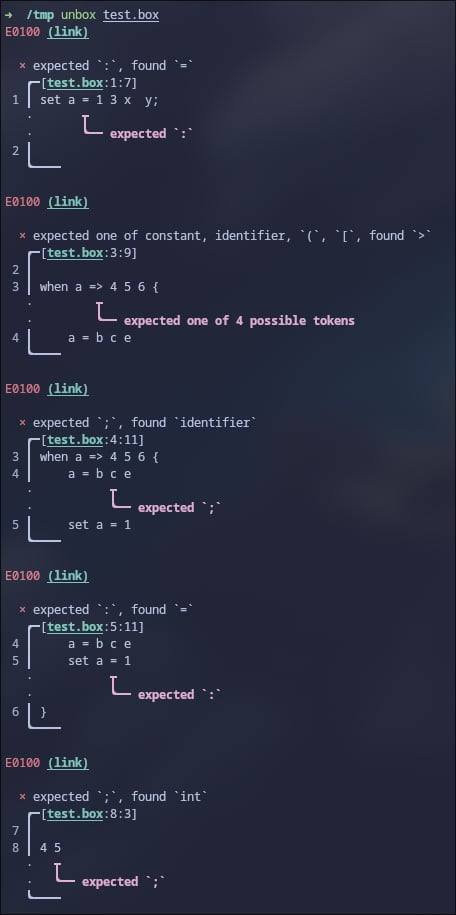
\includegraphics[scale=0.75]{panic-mod-res.jpg}
    \caption{Kết quả thực thi chương trình với lỗi cú pháp}
\end{figure}

\subsection{Xử lý lỗi trong quá trình phân tích ngữ nghĩa và quá trình thông dịch}

    Do quá trình phân tích ngữ nghĩa và quá trình thông dịch được diễn ra đồng thời, xen kẽ với nhau, nên ta sẽ phân tích cả hai giai đoạn này trong một phần. Trong quá trình phân tích ngữ nghĩa, mỗi khi bộ phân tích ngữ nghĩa gặp một lỗi, nó sẽ thông báo lỗi thông qua bộ xử lý lỗi. Bộ xử lý lỗi sẽ hiển thị thông báo lỗi cụ thể và vị trí lỗi trong tệp tin chương trình. Tất cả các lỗi trong hai giai đoạn này đều được xếp vào loại lỗi không thể khôi phục được. Khi gặp lỗi, bộ xử lý lỗi sẽ thông báo lỗi và kết thúc quá trình thông dịch ngay sau đó. Lỗi ở hai giai đoạn này rất đa dạng, từ lỗi kiểu dữ liệu không hợp lệ, lỗi số lượng tham số không hợp lệ, lỗi không tìm thấy biến, lỗi không tìm thấy hàm, ... giúp người dùng dễ dàng xác định lỗi và sửa lỗi.
